\section{Vorlesung 04.11.2016}
\subsection{Kreise}
Sei G(V,E) ein Graph. Teilgraphen H aus G dann beschreiben wir durch deren Kantenmenge F $\subseteq$ E $\Leftrightarrow$ isolierte Knoten in H werden ignoriert\\
isoliert: deg$_H$(x)=0
\\\\
Kreis C - zusammenhängend und deg$_C$(x)=2\\
verallgemeinerte Kreise: kantendisjunkte Vereinigung von Kreisen\\
eulerscher Kreis: zusammenhängende verallgemeinerte Kreise\\
\\
\underline{Bemerkung:} verallgemeinerte Kreise haben überall geraden Knotengrad
\begin{figure}[htp]
\centering
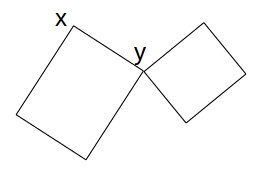
\includegraphics[scale=0.75]{lectures/161104/pix/pic1.jpg}
deg(x)=2\\
deg(y)=4
\end{figure}

\textbf{Theorem (Euler):}
\begin{enumerate}
	\item H ist verallgemeinerter Kreis $\Leftrightarrow$ jeder Knoten geraden Grad
	\item Wenn H zudem zusammenhängend dann gibt es einen geschlossenen Weg der Kanten von H (genau 1 mal) enthält.
\end{enumerate}

\underline{Beweisskizze des Euler-Theorems}\\
\textbf{zu 1:}\\
$\Rightarrow$ erledigt in der oberen Bemerkung\\
$\Leftarrow$ zeige: Sei H zusammenhängend und deg(x) ist gerade für alle Knoten $\Rightarrow$ H ist ein verallgemeinerter Kreis
\\\\
$\rightarrow$ sei u ein beliebiger Startpunkt. Konstruiere einen Weg w in H ausgehend von u
\begin{figure}[htp]
\centering
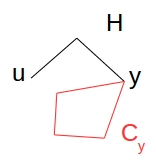
\includegraphics[scale=0.75]{lectures/161104/pix/pic2.jpg}
\end{figure}
\newpage
w erreicht nach endlich vielen Schritten einen bereits benutzten Knoten y zum zweiten Mal.\\
Teilweg von der 1. zur 2. Berührung von y ist ein Kreis, weil dieses Wegstück ein Pfad ist. Nennen diesen Kreis C$_y$.\\
Konstruiere den Graphen H$\backslash$C$_y$=: H'\\
Für H' gilt: deg$_{H'}$(x)=deg$_H$(x)-2 wenn x nicht auf C$_y$ liegt
\\\\
\underline{Also:} In H gibt es einen Kreis C$_y$
\begin{itemize}
	\item H$\backslash$C$_y$ hat wieder nur geraden Knotengrad
	\item H$\backslash$C$_y$ muss aber nicht mehr zusammenhängend sein
	\item außerdem hat H$\backslash$C$_y$ strikt weniger Knoten als H
\end{itemize}

Wiederhole die Zerlegung H $\rightarrow$ H$\backslash$C$_y$ für jede Zusammenhangskomponente von H'
\begin{figure}[htp]
\centering
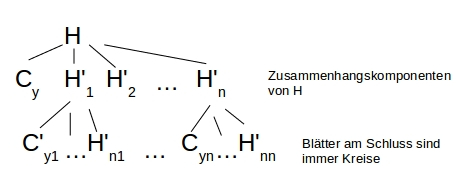
\includegraphics[scale=1.00]{lectures/161104/pix/pic3.jpg}
\end{figure}

$\Rightarrow$ Alle entstehenden Kreise sind Kantendisjunkt. Die Vereinigung der Kreise ist ganz H.
\newpage
\textbf{zu 2:}\\
Seien C$_1$ und C$_2$ zwei Kreise, die wenigstens einen Knoten gemeinsam haben
\begin{figure}[htp]
\centering
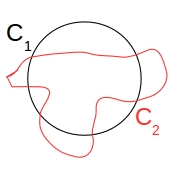
\includegraphics[scale=0.75]{lectures/161104/pix/pic4.jpg}
\end{figure}

\begin{itemize}
	\item Suche einen Startpunkt auf C$_1$ (beliebig!)
	\item Folge C$_1$ bis zum 1. Schnittpunkt mit C$_2$ (=y)
	\item folge C$_2$ $\rightarrow$ das führt zurück nach y
	\item folge C$_1$ zurück zum Startpunkt
\end{itemize}

$\Rightarrow$ diese Vorschrift erzeugt einen geschlossenen Weg (nicht Pfad!) auf C$_1 \cup$ C$_2$ der alle Kanten von C$_1$ und C$_2$ verwendet \textcolor{red}{(wie sind rote Hinweise in Mitschrift zu verstehen???)}\\

\underline{wenn mehrere Kreise beteiligt:}\\
\begin{itemize}
	\item Suche einen Startpunkt auf C$_1$ (beliebig!)
	\item Folge C$_1$ bis zum 1. Schnittpunkt mit Q (=y)
	\item folge Q $\rightarrow$ das führt zurück nach y
	\item folge C$_1$ zurück zum Startpunkt
\end{itemize}

$\Rightarrow$ diese Vorschrift erzeugt einen geschlossenen Weg (nicht Pfad!) auf C$_1 \cup$ Q der alle Kanten von C$_1$ und Q verwendet, d.h. C$_1 \cup$ Q enthalten einen \underline{Eulerschen Pfad}\\

Kreis C$_1$, kantendisjunkte Vereinigung Q von k Kreisen, zusammenhängend die C$_1$ in wenigstens einen Punkt schneidet

Angenommen auf Q gibt es einen Eulerschen Weg (d.h. einen geschlossenen Weg, der jede Kanten von Q enthält) $\rightarrow$ siehe oben \emph{wenn mehrere Kreise beteiligt}
\\\\
Vollständige Induktion nach der Zahl der Kreise in Q.\\
Beweis Fall k=1 (mit k=Anzahl der Kreise), Q ist Kreis, der auch Eulerpfad in Q ist.
\\\\
\underline{Iteration:} k-1=k\\
Wenn Q mit k-1 Kreisen einen Eulerschen Pfad enthält (=Induktionsannahme) dann enthält C$_1 \cup$ Q (k-Kreise) auch einen Eulerpfad $\rightarrow$ \underline{Aussage 2 damit korrekt}

\subsection{Kreisbasen}
Seien H$_1$ und H$_2$ zwei Teilgraphen von G. Dann ist H$_1$ $\oplus$ H$_2$ der Teilgraph von G mit Kantenmenge (H$_1$ $\cup$ H$_2$ $\backslash$ (H$_1$ $\cap$ H$_2$))\\
$\oplus$ heißt auch symmetrische Differenz (XOR)
\begin{figure}[htp]
\centering
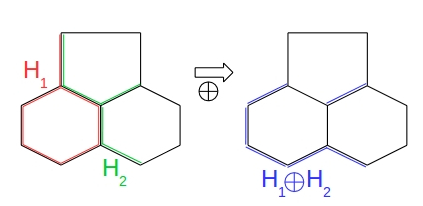
\includegraphics[scale=1.00]{lectures/161104/pix/pic5.jpg}
\end{figure}

\underline{Lemma:} Seien C$_1$ und C$_2$ verallgemeinerte Kreise dann ist C$_1$ $\oplus$ C$_2$ wieder verallgemeinerter Kreis
\\\\
\underline{Beweis:}\\
deg$_{C_1}$(x) = 0 mod 2\\
deg$_{C_2}$(x) = 0 mod 2\\
deg$_{C_1 \oplus C_2}$(x) = 0 mod 2
\\\\
C$_i$(x) = Menge der Kanten in C$_i$ (i=1,2,1$\cup$2) die x enthalten\\
C$_{1 \cup 2}$(x) = (C$_1$(x) $\cup$ C$_2$(x)) $\backslash$ (C$_1$(x) $\cap$ C$_2$(x))\\
$|$C$_{1 \cup 2}$(x)$|$ = $|$C$_1$(x)$|$ + $|$C$_1$(x)$|$ - 2$|$C$_1$(x) $\cap$ C$_2$(x)$|$\\
gerade $\Leftarrow$ gerade + gerade - gerade
\\\\
\underline{Charakteristischer Vektor eines Teilgraphen H}\\

{\LARGE $\chi$}$_H(e)=
	\begin{cases}
		\text{1 wenn } e \in H\\
		\text{0 sonst}
	\end{cases}
$
\\\\
\underline{Lemma:} Sei $\mathcal{H}$ die (ungerichtete) Inzidenzmatrix von G\\
Dann gilt {\large$\mathcal{H}$} $\cdot$ {\Large $\chi$}$_H$=0 $\Leftrightarrow$ H ein verallgemeinerter Kreis in G ist
\\\\
$\bigoplus\limits_{e} \mathcal{H}_{x \cdot e} \cdot \chi_{_H}(e)=0$ für alle Knoten x in G\\
mit $\mathcal{H}_{x \cdot e}$ 1 wenn x Endpunkt von G, 0 sonst
\newpage
Beweis: nachrechnen (Achtung Rechenregeln GF(2)\footnote{\url{https://en.wikipedia.org/wiki/GF\%282\%29}})\\
GF(2)=\{1,0,$\oplus$,\}
\begin{itemize}
	\item 1 $\oplus$ 1 = 0
	\item 1 $\oplus$ 0 = 0 $\oplus$ 1 = 1
	\item 0 $\oplus$ 0 = 0
\end{itemize}

Weil $\mathcal{H} (\chi_{_{H_1}} \oplus \chi_{_{H_2}}) = \mathcal{H} \cdot \chi_{_{H_1}} \oplus \mathcal{H} \cdot \chi_{_{H_2}} = 0$ (wieder \underline{v}erallgemeinerte \underline{K}reise) mit\\
$\mathcal{H} \cdot \chi_{_{H_1}}$=0 und $\mathcal{H} \cdot \chi_{_{H_2}}$=0 weil H$_1$ und H$_2$ v.K.
\\\\
\underline{$\Rightarrow$ verallgemeinerte Kreise bilden einen Vektorraum}
\\\\
Deswegen gilt es einen Basis, d.h. eine Menge von Kreisen B=\{C$_1$,C$_1$,…,C$_{\mu}$\} sodass jeder verallgemeinerte Kreis C dargestellt werden kann als\\
$C=\bigoplus\limits_{i=1}^{\mu} \lambda_i C_i$ mit $\lambda \in \{0,1\}$
\\
$\Leftrightarrow$ jeder v.K. C ist die Summe einer eindeutig bestimmten Teilmenge B$_C \subseteq$ B
\\\\
\textbf{Basis:} minimale Menge von erzeugenden Kreisen
\\
Vektorraum $\Rightarrow$ alle minimal erzeugende Kreismenge sind gleichgroß\\
Zahl Basiskreis ... Dimension \textcolor{red}{?}
\\\\
Menge M=\{C$_1$, ..., C$_\mu$\} von Kreisen (im allgemeinen Vektorraum) heißt linear unabhängig wenn gilt:\\
$\bigoplus\limits_{i=1}^{|M|} \lambda_i C_i$ mit $\lambda \in \{0,1\}\Rightarrow$ $\lambda_i=0$ $\forall i=1 ... |M|$ \textcolor{red}{?}
\\\\
Beispiel:
\begin{figure}[htp]
\centering
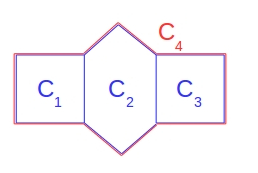
\includegraphics[scale=0.75]{lectures/161104/pix/pic6.jpg}
$\underbrace{C_1 \oplus C_2 \oplus C_3}_{C_4 \oplus C_4 = 0} \oplus C_4=0$
\end{figure}

M=\{$C_1$, $C_2$,$C_3$,$C_4$\} ist abhängig weil $\lambda_1=\lambda_2=\lambda_3=\lambda_4=1$ die Gleichung\\
$\bigoplus\limits_{i=1}^{4} \lambda_i C_i=0$ löst
\\\\
M=\{$C_1$, $C_2$,$C_3$\} ist unabhängiges Argument. Jeder Kreis enthält eine Kante, die in keinem anderen Kreis aus M vorkommt und daher nicht in einer Summe anderer Kreise auftreten kann.
\\\\
\underline{daher nochmal Basis:}
\begin{itemize}
	\item maximale unabhängige Menge
	\item minimale erzeugende Menge
\end{itemize}

\underline{Konstruktion von Kreisbasen:} Kichhoff Basen (strikt fundamental Basen)
\\
Graph G zusammenhängender Spannbaum T von G\\
Für jede Kante $e\notin T$ enthält $T \cup \{e\}$ genau einen Kreis $\rightarrow$ C$_{e,T}$\\
\underline{\textbf{WARUM?}} Seien x,y die Endpunkte von e dann gibt es genau einen Pfad von x nach y in T. Der wird mit e zu genau einem Kreis.
\\
$B_T=\{C_{e,T}\backslash e \in T\}$ ist eine Kreisbasis \textcolor{red}{so richtig? oder $|$ statt $\backslash$}
\\
\underline{Beweis:} zu zeigen
\begin{enumerate}
	\item Jeder Kreis kann als Summe der $C_{e,T}$ erzeugt werden
	\item Die Kreismenge B ist unabhängig
\end{enumerate}

\underline{zu 1.:} Sei Z ein Kreis, z$\notin$B (Z keine Kreisbasis)\\
$\Rightarrow$ Z Summe von Baiskreisen. Wenn e $\in$ Z$\backslash$T dann muss C$_{e,T}$ zu Z beitragen. Wenn e $\notin$ Z$\backslash$T dann e$\in$T gibt es keinen zugehörigen Basiskreis\\
e$\notin$T, e$\notin$Z dann kann C$_{e,T}$ nicht zu Z beitragen\\\\
Also $\bigoplus\limits_{e \in Z\backslash T} C_{e,T}$

\underline{zu 2.:} $C_{e,T}$ enthält nicht e für e,e'$\in$T, e$\neq$e'\\
$\Rightarrow$ jeder Basiskreis enthält einen Kante, die in keinem anderen Basiskreis enthalten ist $\Rightarrow$ \underline{Unabhangigkeit}
\\\\
Wie viele Kreise einthält B (Kirchhoff-Basen)?\\
$|$B$|$ = $|$E$|$-$|$T$|$\\
Kanten in Spannbaum $|$T$|$=$|$V$|$-1 $\Rightarrow$ $|$B$|$ = $|$E$|$-$|$V$|$+1
\\\\
\underline{am Allgemeinen:} $|$B$|$ = $|$E$|$-$|$V$|$+C(G) mit C(G)= Anzahl der Zusammenhangskomponenten\\
 - nicht notwendig zusammenhängend
\\\\
\underline{Bemerkung:} Die Kreise aus der "Eulerzerlegung" eines Graphen mit geraden Knotengrad bilden
\begin{itemize}
	\item unabhängige Menge da kantendisjunkt
	\item aber normalerweise \underline{keine} Basis
\end{itemize}

\newpage
\underline{Beispiel:}
\begin{figure}[htp]
\centering
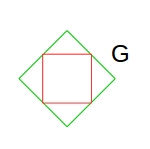
\includegraphics[scale=1.00]{lectures/161104/pix/pic7.jpg}
$| \epsilon |$=2 mit $\epsilon$=Eulerkreise\\
$|$B$|$ = $|$E$|$-$|$V$|$+1 = 12 - 8 + 1 = 5\\
Basis für G: \textcolor{green}{4 Dreiecke} + \textcolor{red}{1 Viereck} = 5
\end{figure}

\underline{linear unabhängig?}\\
für Dreiecke ja da Kantendisjunkt (wäre eine alternative Eulerzerlegung)
\\\\
\textbf{bei Viereck?}\\
\begin{figure}[htp]
\centering
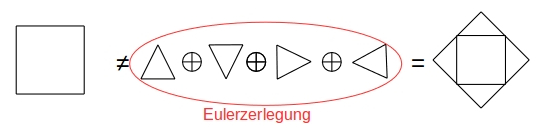
\includegraphics[scale=1.00]{lectures/161104/pix/pic8.jpg}
\end{figure}

Viereck kann nicht durch Summe der Dreiecke dargestellt werden $\Rightarrow$ linear unabhängig
\\\\
Gibt es einen Spannbaum der für G die Kirchhoffbasis (4 Dreiecke + Viereck) erzeugt?\\
$\Rightarrow$ nein, da jeder Spannbaum der das Viereck erzeugt kann eines der 3-Ecke nicht erzeugen